\noindent Previous experimental and numerical studies in micro-circulation have demonstrated that certain physiological phenomena are associated with the motion of RBCs across diverging bifurcations (see Figure \ref{FluidMechanicalPhenomena}). In these diverging bifurcations, the RBC partitioning does not necessarily distribute proportionally to the partition of blood flow which leads to a high degree of heterogeneity within the network of micro-vessels. These phenomena contribute to the formation of a cell-free layer (CFL) near the interior vessel walls which not only cause lateral migration of RBCs away from vessel walls but also defines the distinctive blood flow properties in micro-vessels.\cite{AnnualReview} 

\begin{figure}[H]
\centering
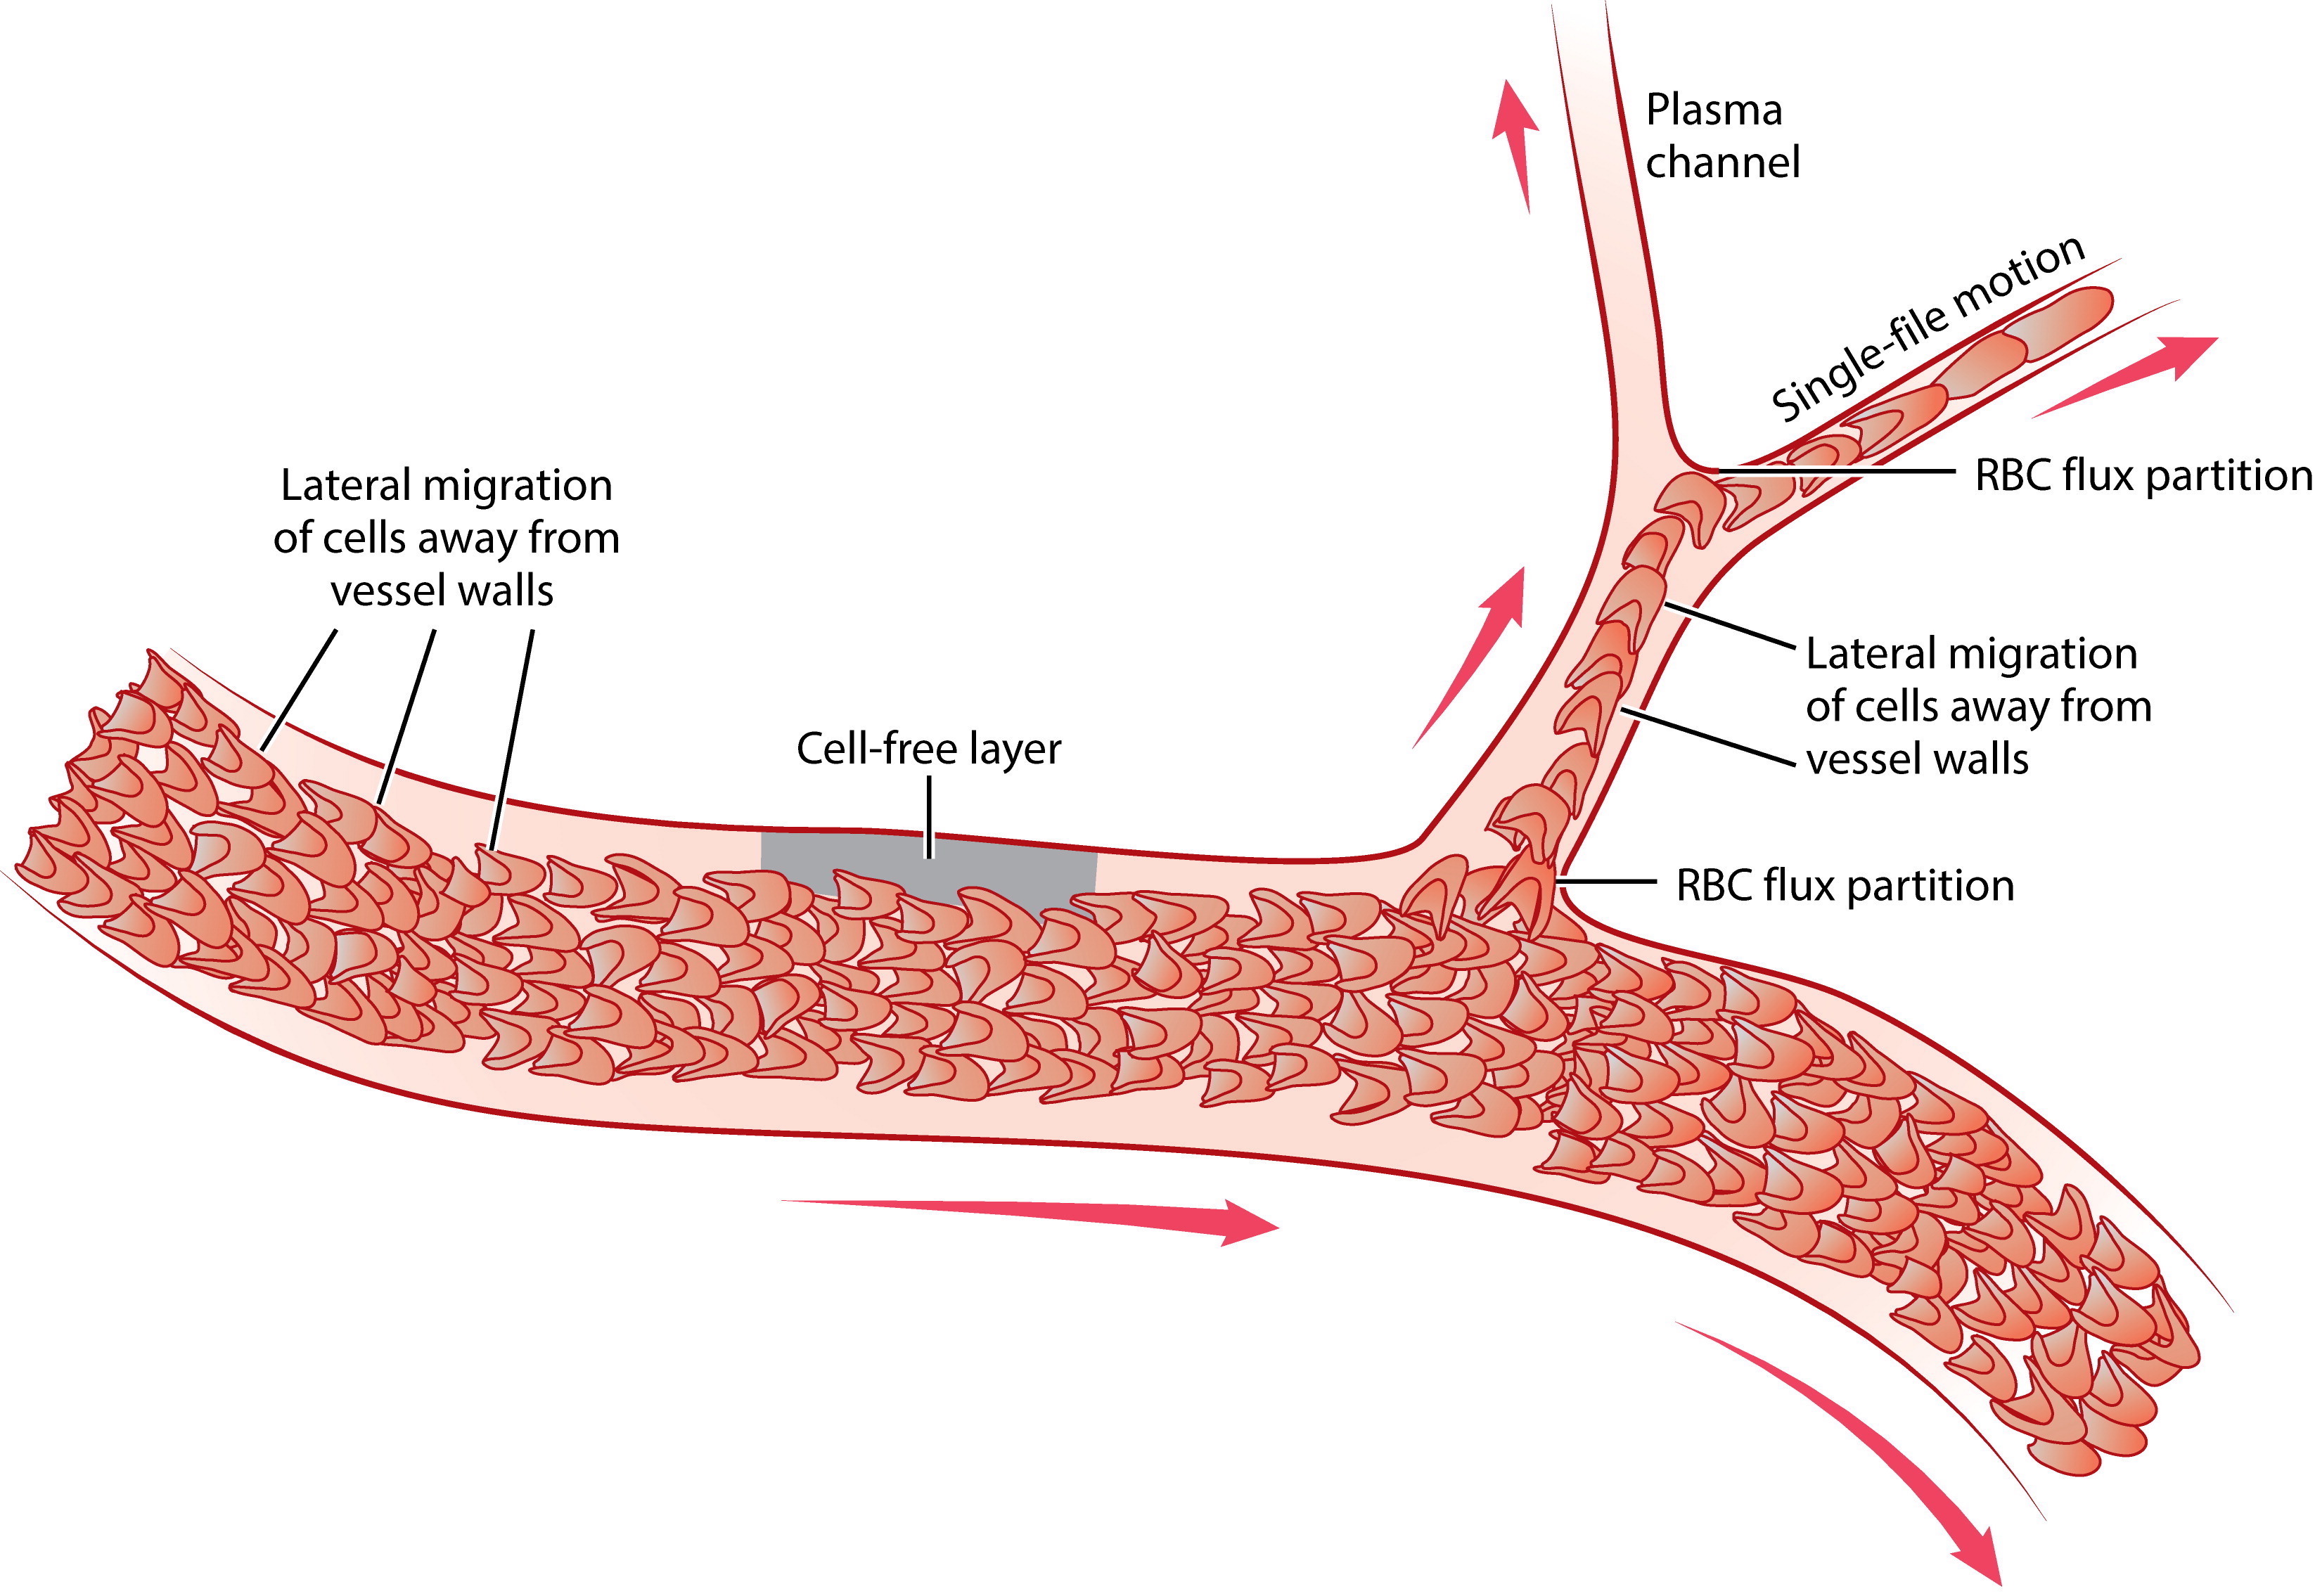
\includegraphics[width=0.85\textwidth]{images/PlasmaSkimming.jpeg}
\caption{\textit{Different fluid mechanical phenomena caused by uneven distribution of red blood cells at diverging bifurcations.\cite{AnnualReview}} \label{FluidMechanicalPhenomena}}
\end{figure}


\noindent One example is the tendency for RBCs flowing near the vessel walls to migrate away from the walls due to their deformability, hence forming a cell-free layer near the walls and altering the RBC distribution downstream.\cite{PhysRevLett} Another plausible physical mechanism is due to the Poiseuille velocity profile's curvature in tube flow which causes the tendency of RBC migration towards the centre line of the flow (assuming wall effects are neglected).\cite{2020Charles} However, the effect from the velocity profile curvature only dominates significantly under dilute suspensions and not concentrated suspension conditions. This is because both the shear-induced dispersion effect and cell-to-wall interactions are more prevalent mechanisms that govern the radial distribution of RBCs in microvascular networks.\cite{CoupierG2008Nlmo} The following subsections highlight the different plausible mechanisms that contribute to the radial distribution of RBCs in multi-file flows.


\subsubsection{Cell-to-Cell Interactions}
\noindent An investigation of the effects of cell-to-cell mechanical interactions is important to understand the RBC partitioning behaviours in diverging bifurcations. In reference to a 2D computational modelling study conducted by Barber et al.\cite{Barber2011SimulatedPartitioning}, three main types of two-cell interactions were found that can affect the RBC partitioning. The first interaction is a "trade-off" mechanism where the front cell enters a child branch, and the following cell enters the opposite child branch. For the second interaction, it is a "following" mechanism that occurs when the rear cell enters the same branch as the front cell. Lastly, "herding" is the third mechanism observed where the front cell enters the same branch as the rear cell.  \\

\noindent The "trade-off" mechanism appears to occur most frequently unlike the other two mechanisms due to continuity of flow and conservation of mass law. This causes a tendency towards having a more uniform haematocrit partitioning in the downstream branches as haematocrit increases although the opposing effects of "following" and "herding" mechanisms do slightly counteract this tendency.\cite{Barber2011SimulatedPartitioning} However, do take note that these mechanisms mentioned above are only considering the effects of two-cell interactions in 2D systems and under dilute suspension conditions. Whereas under physiological conditions with 40\% hematocrit, the collisions between RBCs will occur more frequently due to the strong hydrodynamic interactions that oppose the migration to the centreline and cause the RBCs distribution to broaden in parent branches.\cite{PRIES198981} Therefore, there is a greater tendency for concentrated RBC suspensions under shear flow conditions to migrate across the flow and towards the walls in the of decreasing concentration. This phenomenon is referred to as the shear-induced dispersion effect.\cite{Leighton1987MeasurementSpheres, Pranay2012, HariprasadSecomb2014} 



% This will fluctuate the lateral velocities and drive a diffusion-like motion of the particles, with a net flux down the concentration gradient. Therefore, the development of quantitative models are required to observe other types of interactions involving multiple cells at higher haematocrit and in 3D systems. 


\subsubsection{Cell-to-Wall Interactions}
\noindent On the other hand, previous studies of the motion of RBCs under shear flow near a solid boundary have also demonstrated that under the Stokes flow regime, the RBC suspensions in tubes tend to migrate away from the interior walls in 3D simulations.\cite{CoupierG2008Nlmo, DoddiSaiK2009Tcmo} This is primarily due to the effects of RBC deformability to cell trajectories that causes this migration phenomenon to occur\cite{PhysRevLett}. However, the complete mechanistic understanding of this phenomenon is difficult as multiple effects are involved. This is because there is no concrete evidence to prove that the deformable RBCs close to the walls will consistently migrate away from the wall in all scenarios. \\

\noindent However, there are certain distinct observations found in several experiments that do partially answer the physical mechanisms related to this migration phenomenon. For dilute suspensions under shear-flow conditions, tank-treading motions were observed in numerous experiments where these close-wall tank- treading RBCs tend to migrate away from the interior walls due to hydrodynamic lift force which leads to axial drifting.\cite{Olla_1997A, Olla_1997B, PhysRevLett.83.876, PhysRevLett2002, PhysRevLett} Therefore, this gives rise to the development of CFL where it serves as a lubricant film that decreases the apparent viscosity of blood in the tube and also has prominent implications for blood flow in micro-circulation.\cite{feng_weinbaum_2000, CharlesPhDThesis2020}


% If the suspending medium has a viscosity similar to that of plasma, RBCs exhibit tumbling motions with the vorticity vector of the shear flow as the axis (Keller & Skalak 1982, Barthes-Biesel 2016). Migration away from the wall is still observed in this case (Grandchamp et al. 2013).

% https://journals.aps.org/prl/abstract/10.1103/PhysRevLett.98.188302
% a swinging motion of the RBC was discovered in several experiments and this motion was characterised by an oscillating inclination angle on top of the classic tank-treading motion


\subsubsection{Initial RBC Distribution in Parent Branch}
\label{InitialRBCDistributionInPB}
\noindent Previous experimental studies have established several well-known models\cite{PRIES198981, GuibertR2010ANAt, Gould2015HematocritNetworks, LeeTae-Rin2017Gpsm} that describe the plasma skimming effects under a central assumption of axisymmetric haematocrit profile in the parent branch of each bifurcation. However, substantial haematocrit asymmetry has always been observed in the parent branches across numerous studies.\cite{Zhou2021EmergentBifurcations, 2020Charles} This suggests that without specific knowledge of the cross-sectional RBC distribution in a given branch, it will be challenging to have an accurate prediction of the downstream blood flow behaviours across the networks. Furthermore, a recent study in tumour vascular networks has pointed out other sources of haematocrit asymmetry such as the reduced interbifurcation distance and complex vessel topology which drives oxygen heterogeneity in solid tumours.\cite{Bernabeu2020AbnormalOxygenation} Apart from haematocrit asymmetry, the uneven velocity profile in capillary vessels can also occur as the parabolic velocity profile can become skewed over time due to the presence of RBCs.\cite{2020Charles, JosephAby2019Isbf, Balogh2018, Balogh2017DirectNetworks} Therefore, both asymmetries in velocity and haematocrit profiles in the parent branch can significantly affect the radial distribution of RBCs in the downstream branches and across the microvascular networks.


\subsubsection{Cellular Mechanisms: Lingering \& Jamming}
\noindent The rapid improvement in computational studies has enabled researchers to identify and analyse cellular-scale mechanisms underlying the time-dependent partitioning behaviours. Recent studies of RBC partitioning through simplified and complex geometries\cite{wang_sui_salsac_barthes-biesel_wang_2016, Balogh2018, Balogh2017DirectNetworks} have observed cell lingering and jamming effects occurring across the microvascular networks. The RBCs lingering dynamics at vascular bifurcations results in temporary and partial obstructions to the blood flow in both child and parent branches as this also lead to cell jamming at the bifurcations. As a consequence of these mechanisms, this leads to reverse partitioning behaviours occurring across the microvascular networks.\cite{Balogh2017DirectNetworks} Furthermore, the mechanisms are also associated with the asymmetric distribution of RBCs in the downstream bifurcations due to the pilling up of RBCs at the upstream bifurcations which results in a haematocrit reduction in the child branches.\cite{Balogh2018} (see Figure \ref {CellularMechanisms} for illustration purposes.)

\begin{figure}[H]
\centering
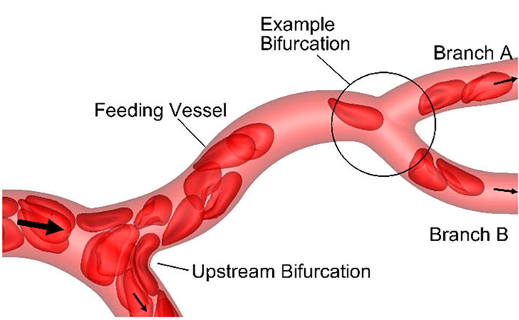
\includegraphics[width=0.85\textwidth]{images/CellularMechanisms.png}
\caption{\textit{An illustration of a reverse partitioning behaviour due to cellular mechanisms in a successive bifurcation from micro-vascular networks. The pilling-up of RBCs in the upstream bifurcation affects the RBCs entering the feeding vessel to shift towards the left-hand side of the vessel which results to increasing the fractional RBC flux in branch A.\cite{Balogh2018}} \label{CellularMechanisms}}
\end{figure}

\noindent However, these results from recent studies\cite{Balogh2018, Balogh2017DirectNetworks, KihmAlexander2021LDiM} have not yet been compared to a detailed analysis of the lingering effects in \textit{in vivo} experiments. All of the lingering effects observed were described based on \textit{in silico} experiments which lack the proper quantification and full understanding of this lingering effect in \textit{in vivo} experiments. Therefore, further investigations will be required in the future to elucidate the fundamental dynamics of the cell lingering effects under \textit{in vivo} conditions. This is because the impact of cell lingering on the blood flow behaviour can lead to severe implications on the entire micro-vascular network as it can significantly disrupt the radial distribution of RBCs across multiple micro-vessels.  



% We have provided evidence to show that these lingering events cause a breakup of trains of RBCs as well as redistribution in the branching vessels. Even though these effects seem to be rather fine grained, the impact on the whole organism may be severe, given the importance of blood flow to the health state.x


\subsubsection{Effects of the Endothelial Surface Layer}
\noindent According to numerous \textit{in vivo} investigations\cite{Pries2000TheLayer, ReitsmaSietze2007Tegc, WeinbaumSheldon2007Tsaf, SmithMichaelL2003Nmra, A.R.Pries2005Mbvi}, there was strong evidence of endothelial surface layer (ESL) existing near the interior surfaces of the blood vessels (see Figure \ref{EndothelialSurfaceLaye}). It was suggested that the interactions between the plasma and membrane-bound glycocalyx were responsible for the formation of ESL.\cite{Pries2000TheLayer} The ESL consists of squamous endothelial cells, which reduces the effective width of the lumen and largely hinders the flow of plasma and RBCs.\cite{Pries2000TheLayer, WeinbaumSheldon2007Tsaf} This shows that the presence of the ESL will have a significant effect on the haemodynamic components in micro-circulation such as flow resistance where the effect amplifies in micro-vessels especially for extremely narrow diameters which substantially increases the flow resistance. Additionally, results from Pries et al.\cite{PriesAR1990BFiM, PriesAR1994RtBF, Pries2000TheLayer} experiments have proven that the presence of ESL greatly affects the haematocrit distribution in complex blood flow networks. Therefore, this highlights the importance of considering ESL in \textit{in silico} experimental modellings as it will aid researchers to gain a further understanding of the mechanical interactions between the RBCs and ESL in complex microvascular networks. 

\begin{figure}[H]
\centering
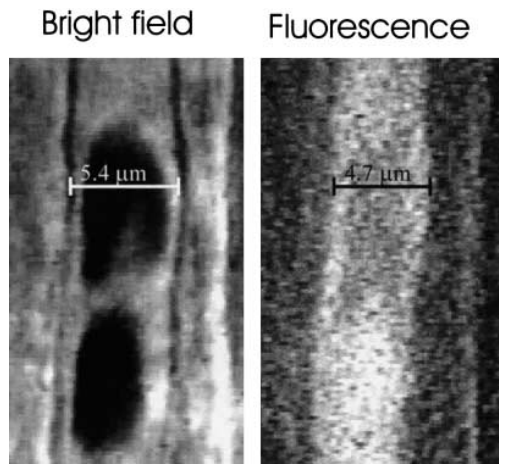
\includegraphics[width=0.7\textwidth]{images/EndothelialSurfaceLayer.png}
\caption{\textit{Existence of the endothelial surface layer via observations from a capillary in the hamster cremaster recorded during intravital microscopy. Under a bright field illumination shows the anatomical width of the capillary (Right) while under a fluorescence illumination identifies the width of the plasma column (Left). The difference suggests the presence of the endothelial surface layer.\cite{Pries2000TheLayer}} \label{EndothelialSurfaceLaye}}
\end{figure}


\subsubsection{Presence of Other Suspended Particles}
\noindent Although RBCs and plasma are the two main dominant components in blood, there are several other biologically important types of cells that should be considered such as white blood cells (WBC) or platelets.(see Figure \ref{BloodComponents}) To perform their biological functions, the ability for these particles to reach the micro-vessel walls is crucial as the WBCs are responsible for the body's responses to injuries and infections while the main function for platelets is to stop bleeding from damaged blood vessels. Therefore, the fluid dynamic interactions with RBCs affects these particles lateral motion within micro-vessels as numerous experiments\cite{GoldsmithHarryL1984Moli, NobisU1985Rdow, TangelderG1985} and computational studies\cite{FedosovDmitryA2014Wbcm, FreundJonathanB2007Lmia, VahidkhahKoohyar2014PDiT, MehrabadiMarmar2015ACMf, PhysRevLett.108.028104} have observed that both of WBCs and platelets are preferably distributed near the walls of the vessels. This migration of RBCs away from vessel walls primarily depends on the RBC's deformability which also induces the outward migration of more rigid particles like WBCs and platelets.\cite{PhysRevLett.109.108102} Therefore, this highlights the dependence of other suspended particle migrations on the hydrodynamic interactions of RBCs within the vessel walls as this affects the radial distribution of RBCs across the microvascular networks.

